
\documentclass[journal]{IEEEtran}

% *** GRAPHICS RELATED PACKAGES ***
%

  %\usepackage[pdftex]{graphicx}
  \usepackage{graphicx}
  \usepackage{caption}
  \usepackage{subcaption}
  \usepackage{amsmath}
  % declare the path(s) where your graphic files are
 \graphicspath{{../pdf/}{../jpeg/}}
  % and their extensions so you won't have to specify these with
  % every instance of \includegraphics
   \DeclareGraphicsExtensions{.pdf,.jpeg,.png}
\usepackage[export]{adjustbox}
\usepackage{float}

\usepackage[section]{placeins}

% correct bad hyphenation here
\usepackage{fixltx2e}
 \usepackage{cite} 
\usepackage{url}


\usepackage{epstopdf}

\epstopdfDeclareGraphicsRule{.gif}{png}{.png}{convert gif:#1 png:\OutputFile}
\AppendGraphicsExtensions{.gif}

\setcounter{totalnumber}{5}
\setcounter{topnumber}{5}
\setcounter{bottomnumber}{5}
\renewcommand{\topfraction}{1}
\renewcommand{\bottomfraction}{1}

\begin{document}
%
% paper title
% can use linebreaks \\ within to get better formatting as desired
% Do not put math or special symbols in the title.
\title{Project: 3D Pose Estimation from 2D Projections}
%
%
% author names and IEEE memberships
% note positions of commas and nonbreaking spaces ( ~ ) LaTeX will not break
% a structure at a ~ so this keeps an author's name from being broken across
% two lines.
% use \thanks{} to gain access to the first footnote area
% a separate \thanks must be used for each paragraph as LaTeX2e's \thanks
% was not built to handle multiple paragraphs
%

\author{Richard (Alex) Showalter-Bucher\\Benjamin Yu}


\maketitle

\section{Introduction}
In this project, we explored the application of machine learning to the problem of estimating an object's 3D position and orientation, known as a pose, from a 2D projection. Being able to accurately perform this estimation has applications in several disciplines including Computer Vision, Photogrammetry, and Robotics\cite{Robust_PNP}. A notable application is object tracking in virtual reality systems (VR), such as the HTC Vive and Oculus Rift. Both of these systems estimate 2D angular locations of reference points on the objects being tracked to determine the object's pose.

For a system like the HTC Vive, this measurement is done directly via time of arrival of laser sweeps on reference points which are photodiodes. (Fig \ref{fig:vive}) In the case of the Oculus Rift, a camera is used to identify predetermined reference points (IR LEDs) before estimating the 2D angular location. This is done by blinking each LED in a specific pattern which is observed by a camera. (Fig \ref{fig:oculus}) After the reference points are identified they are centroided to determine their angular location on the focal plane. Once the 2D angular locations are estimated a Perspective N-Point method is applied to estimate the objects pose. In the next subsection we discuss what this method in more detail. 


\begin{figure}
	\hspace{-10 ex}
	\begin{subfigure}{.3\textwidth}
		\centering
		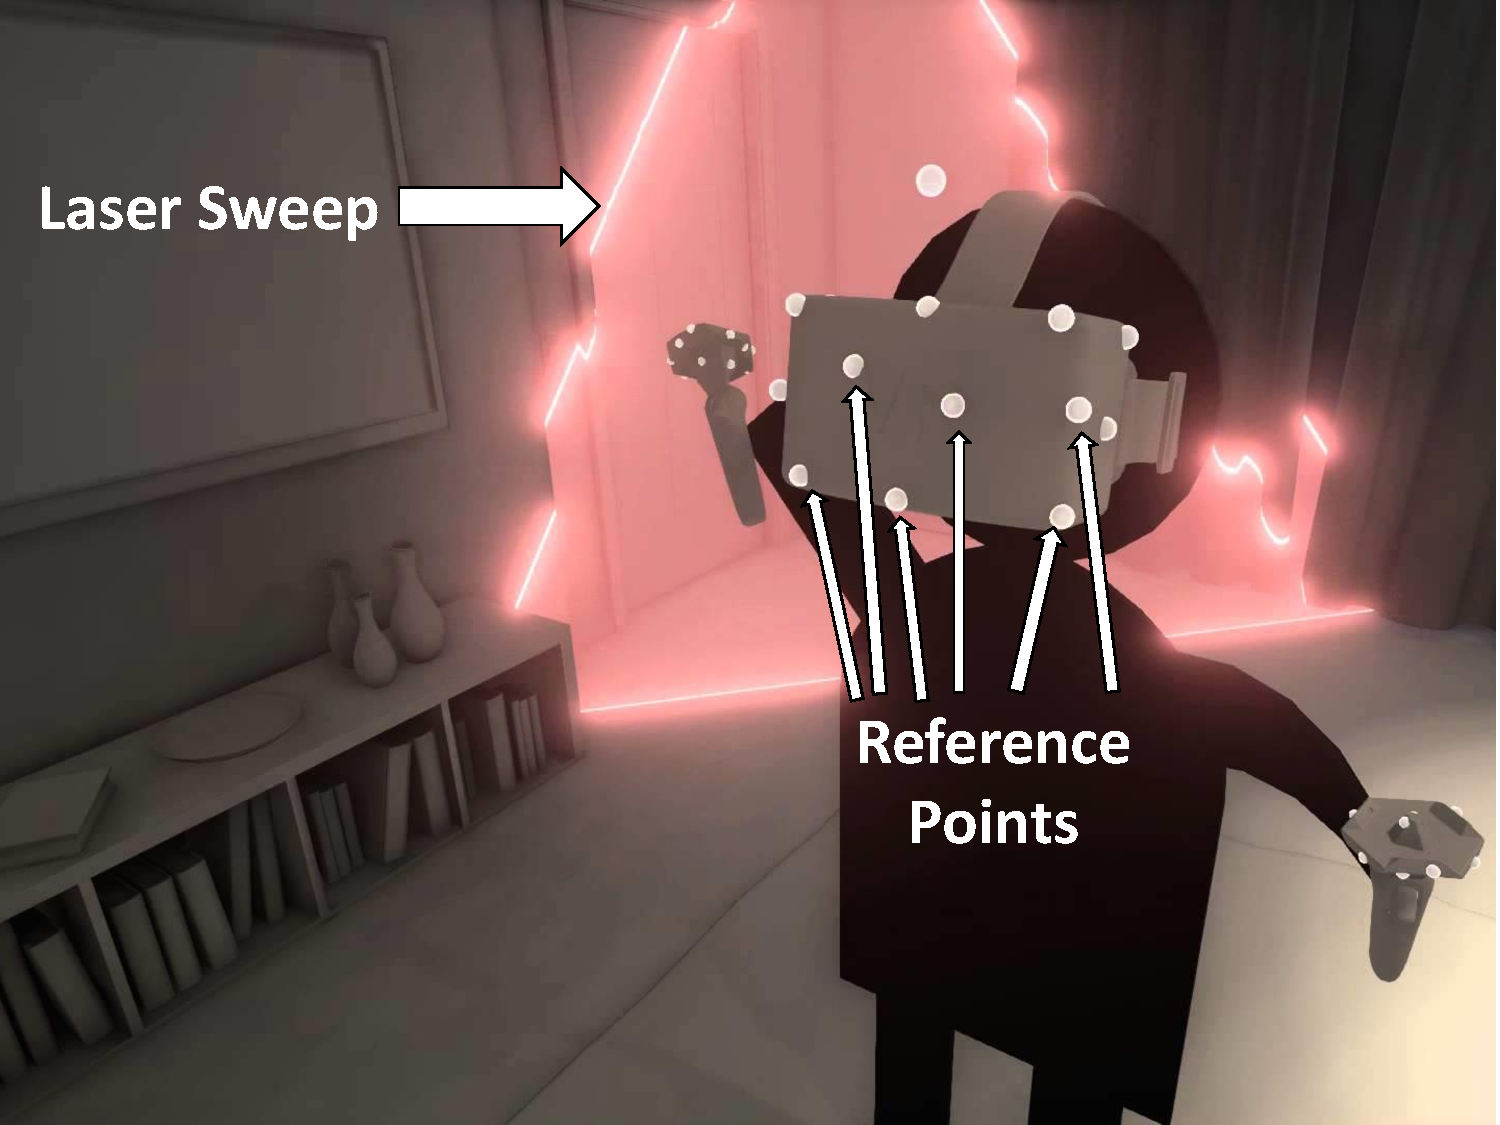
\includegraphics[width=.9\linewidth]{vive}
		\caption{HTC Vive\cite{vive_image}}
		\label{fig:vive}
	\end{subfigure}%
	\begin{subfigure}{.3\textwidth}
		\centering
		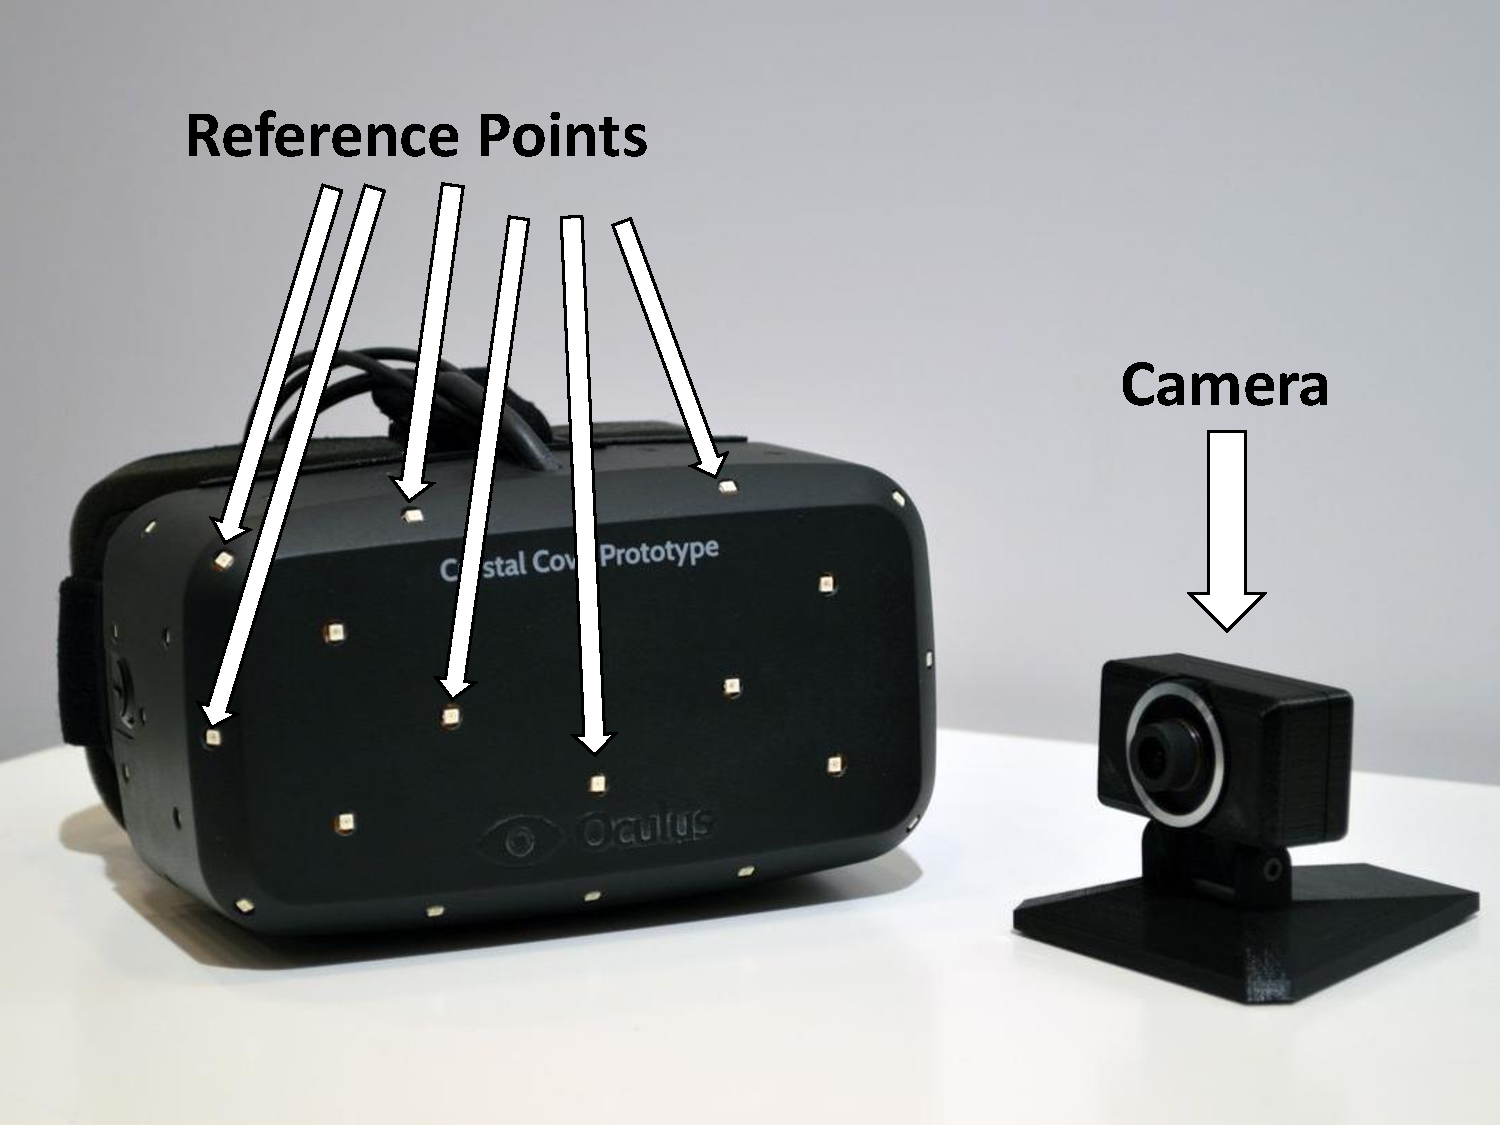
\includegraphics[width=.9\linewidth]{oculus}
		\caption{Oculus Rift\cite{oculus_image}}
		\label{fig:oculus}
	\end{subfigure}
	\caption{Left: HTC Vive's laser sweep with reference points. Right: Oculus Rift's camera with reference points}
	\label{fig:Vive and Oculus}
\end{figure}


\subsection{Perspective N-Point (PnP) Method}
The problem of estimating an objects 3D pose from 2D projections of known reference points is referred to as the "Perspective N-Point" problem. (PnP) 
Common approaches to this problem involve directly or iteratively solving a system of equations\cite{EPnP}. While these approaches can be very precise with the well defined reference points (Minimum of 4 non co-planar points for a non-ambiguous solution), there are usually trade-offs between accuracy and compute time. Direct solvers of these system of equations can be performed computationally fast, but may not be robustly accurate. On the other hand, iterative methods tend to be slower but more robust. A well-formed hybrid of these solvers can be both fast and robustly accurate for well defined points. One of these methods was used to baseline our performance using machine learning algorithms. That method is discussed in more detail in the Baseline Performance EPnP section.



\subsection{Motivation for Applying Machine Learning}
We wanted to implement and test several machine learning techniques to see how they fair with handling the pose estimation problem. There were three different types of techniques we used: SVM Regression, Feed-Forward Neural Networks (FFNN), and Convolutional Neural Networks(CNN). 

We used two different datasets to train our models: raw RGB image data and 2D projections of geometric reference points from an object.
These data types are similar to the raw and processed data, respectively, of the Oculus Rift system. 

Using the reference point data, we were curious if we could match the performance of the PnP method and, if we could obtain similar performance using many points, determine if pose regression using machine learning was robust using less than 4 points (the limitation for non-ambiguous solutions using PnP). Due to the sparsity of this type of data, set we did not train a CNN with it; we tested this type of data only on the SVM and FFNN. 

For the raw image data, we were curious if we could train our models such that they could directly estimate the poses of objects without the need to perform multiple processing steps such as centroiding. If this method worked robustly, then tracked objects may be able to remove explicit defined reference points which would allow for a more cost effective and general solution to the pose estimation problem. 
 
 We also note the use of PnP algorithms require that the reference points, no matter how their locations are measured, are only useful if their exact relative geometry to one another. That is, the PnP algorithms are given knowledge of what the object looks like. In the case our machine learning algorithms, the geometry of the objects are not specified, and must be learned during the training phase. The challenge of tracking objects would then be free of the problem of getting exact geometric measurements.
 
Unfortunately, we found that none of our techniques met the performance of the PnP.  We were hoping to get comparable results to PnP methods but found that the estimations from all data sets were significantly worse than the PnP. We discuss this in more detail in each techniques respective section.

In the next section we discuss our data set and how it was generated. 


\section{Data Set Generation}

To test our machine learning and baseline PnP algorithm we generated two data sets. Each dataset contains versions of a cube, a cone, and a sphere in 500 randomly generated poses. (So each dataset contains 1500 total different samples.) Each pose contains a 3D translation and then yaw, pitch, and roll rotations.

\subsection{Geometric Data Points}

The first data set consists of the projected 2D locations of geometric points from the various shapes. We defined a set of 3D points on the surfaces of the cube, the cone, and the sphere. These base shapes were centered around the origin of our coordinate system. Then, a randomly generated translation and rotation (a pose) was applied to the points. Finally, the points were projected onto a 2D image using a sixty degree field of view.

The geometry of the world was set in a right-handed coordinate system. The camera is at the origin and points along the negative z-axis, so that the x-axis points to the right, and the the y-axis points up (from the point of view of the camera).

The base geometry of each shape was chosen to to have a characteristic dimension of 1.0. The sphere had a diameter of 1.0. The cone had a diameter of 1.0 at its base, and a height of 1.0. The cube had sides of length 1.0. The rotations were allowed to vary uniformly through the space. Yaw varied between 0 and 360 degrees. Pitch varied between positive 90 and negative 90 degrees. Roll varied between 0 and 180 degrees. Those spans are enough to specify any 3D rotation. The x and y of the coordinates of the translation were uniformly distributed between -1.5 and +1.5. The z coordinated varied between -4.33 and -1.7320. This z range placed our shapes at a distance from the camera so that they took up roughly one fifth to a third of the total FOV. We note it was possible for a shape to be half off the image.

The math for applying our random pose, and then projecting our points onto a 2D image follow the vertex processing of OpenGL 1.0. We start with our points from the base shape. These are converted to homogeneous coordinates, which are 4-vectors of the form:

**EQUATION FOR 3D POINT IN HOMOGENOUS COORDINATES**

The benefit of this coordinate system is that both translations and rotations can be written as a matrix multiplication. We create one matrix for the translation, as well as for each of the yaw, pitch, and roll rotations. Finally, we calculate a projection matrix which defines a frustum that represents the field of view of the camera.

**Figure of frustrum**

We then calculate the final locations of the points:

**Equation of rotation**

We normalize these coordinates, by dividing each element of the 4th component of each vector. These normalized coordinates have the property that every point inside that frustum has x, y, and z coordinates in [-1, 1]. Anything else is out of the FOV.

We also calculated the occlusion of each of these points. The final points have z-coordinates, and by defining a set of triangles on the surface of each shape, it is possible to see if a point is blocked by some surface segment of the shape. In the end we record only the location of the projected points on the x-y plane and if the point was occluded.

**FIGURES OF SHAPES**

\subsection{Image Data Set}
Our second data set consisted of full bitmap images of posed cubes, cones, and spheres on a black background. We used the GLUT library to speed our creation of these scenes with OpenGL. Like before, we created 500 random poses of each of the three shapes. The math implemented is the same as in the geometric point case, but of course, OpenGL will render a full scene after transforming the shape vertices.

We applied a texture to our shapes. We chose a high-res version of the Earth from NASA public release. We figured this texture was interesting and also asymmetric. Lack of symmetry is beneficial, as for example, it's possible to, for example, determine which face of the cube you are observing; each face will have a unique part of the Earth on it.

We rendered 64x64 24-bit RGB images and saved them in BMP format. The images are saved unnormalized, but we applied normalization in our algorithms.

**FIGURES OF IMAGE SHAPES**

\section{Baseline Performance of EPnP}

 As a baseline to the performance of the 3D estimation, we used a method referred to as Efficient PnP (EPnP). The implementation of the solver used was included as part of a paper by Lepetit et al\cite{EPnP}. This method is a hybrid method between a direct and iterative solver. In first part of the algorithm, a weighted sum of four virtual points are calculated from n observed reference points. These four virtual points are then used in the direct solver which gives an initial guess of the solution. This guess is then fed into a Gauss-Newton iterative solver which reduces the overall errors in the guess. Overall this implementation's computational cost is linear in terms of the number of reference points.
 
 Results of this method for our geometric reference point data set are shown in Table \ref{EPnP_Table}. Overall the performance of this calculation is robust to some level of noise as long as the points are non-coplanar. A notable issue with this method is seen in cases where the points are co-planar. For example, if the reference points on the base of the cone are the only reference points visible then the direct solver has an issue getting a reasonable initial guess to feed the Gauss-Newton solver.
 
 **(Show figure of examples?)**
 
 This method is great for cases where there the reference points are well defined and non-coplanar. It should be noted that this method also has a strict assumption that the reference points are on a rigid body. This is due to the fact that the 3D geometry of the reference points must be known beforehand to feed to the algorithms. 
 
 

\begin{table}[h]
	\caption{EPnP Performance: Measure Errors = 0, 0.05, 0.1 degs }
	\label{EPnP_Table}
	\centering
	\begin{tabular}{|c|c|c|c|c|}
		
		\hline
		\multicolumn{5}{|c|}{Cone Error} \\
		\hline
		Points: & All & Non-Occluded & 4 & 3\\
		\hline
		RMS & \multicolumn{1}{|l|}{9E-13}  &  &  &\\
		MAX & 6E-12| & &  &\\
		MIN & 2E-14| & &  &\\
		\hline
		\multicolumn{5}{|c|}{Cube Error} \\
		\hline
		Points: & All & Non-Occluded & 4 & 3\\
		\hline
		RMS & 2E-13| &  &  &\\
		MAX & 3E-12 & &  &\\
		MIN & 4E-15 & &  &\\
		\hline
		\multicolumn{5}{|c|}{Sphere Error} \\
		\hline
		Points: & All & Non-Occluded & 4 & 3\\
		\hline
		RMS &  &  & &\\
		MAX &  & &  &\\
		MIN & & &  &\\
		\hline
		
		
	\end{tabular}
\end{table}

\section{SVM Regression}

\subsection{Implementation}

\subsection{Performance on Reference Point Data}

\subsection{Performance on Raw Image Data}

\subsection{Implementation}

\subsection{Performance on Reference Point Data}

\section{Feed-Forward Network (FFNN)}

\subsection{Implementation}

\subsection{Performance on Reference Point Data}

\subsection{Performance on Raw Image Data}

\section{Convolutional Neural Network (CNN)}
We explored using a convolutional neural network on our image data only. This is because CNNs have the ability to relate features locality which makes sense for image data, but does not really help with low dimensionality we see in the point reference data.  

\subsection{Implementation}
We implemented our CNN using a GPU version of TensorFlow. Similar to homework 3, we had an input layer, multiple convolution and pooling layers, a hidden layers, and an output layer.(See Figure ....) 

For the input layer we took each channel(RGB) of in the image and normalized the pixel values such that they could only lay within -0.5 to 0.5. The size of our input layer corresponded to the number of pixels times the number of channels. For the output layer, we used 12 nodes. There were three nodes that represented the 3D position of the object and nine nodes that represented the objects orientation as a direction cosine matrix. We did not apply any activation function the output layer since we were attempting to perform regression and not classification. 

The number of layers, nodes, filter size and stride was tunable hyperparameters for the convolution, pooling layers. For the standard hidden layers, the number of layers and nodes were a tunable parameter. The convolutional and hiddens layer both used Relu activation functions, while the pooling layers used maximum operation as activation functions. 



\subsection{Training}
For training the data, we used a standard L2 Loss function as well the same gradient descent method used in homework 3. 

Since we were not totally sure the best hyperparameters to use for the data set, we decided to implement version of coordinate ascent to attempt to maximize performance. 
In each iteration of coordinate descent we ran through the 

\subsection{Performance on Raw Image Data}


\section{Summary}


\begin{thebibliography}{10}
	
	\bibitem{Robust_PNP} 
	S. Li, C. Xu and M. Xie. \textit{A Robust O(n) Solution to the Perspective-n-Point Problem}, in IEEE Transactions on Pattern Analysis and Machine Intelligence, vol. 34, p. 1444-1450, 2012.
	
	\bibitem{EPnP} 
	V. Lepetit, F. Moreno-Noguer and P. Fua. \textit{EPnP: An Accurate O(n) Solution to the PnP Problem}, in International Journal Of Computer Vision, vol. 81, p. 155-166, 2009.
	
		\bibitem{vive_image} 
	Image Source: \\\texttt{https://i.ytimg.com/vi/J54dotTt7k0/maxresdefault.jpg}
	
	
	\bibitem{oculus_image} 
	Image Source: \\\texttt{http://www.roadtovr.com/wp-content/uploads/2014/01/oculus-rift-crystal-cove.jpeg}
\end{thebibliography}

% For peer review papers, you can put extra information on the cover
% page as needed:
 \ifCLASSOPTIONpeerreview
 \begin{center} \bfseries EDICS Category: 3-BBND \end{center}
 \fi



% For peerreview papers, this IEEEtran command inserts a page break and
% creates the second title. It will be ignored for other modes.
\IEEEpeerreviewmaketitle




   
\end{document}


%Example figure syntax

%\begin{figure}[h]
%\centering
%  \noindent
%  \centering{\hspace{-8 ex} \includegraphics[width=3in]{layers2}}
%  \caption{Boreholes and soil profile with measurements depths.}\label{Fig1Label}

%\end{figure}


%Example equation syntax
%\begin{equation}\label{eq:wavenum}
%k(z) = 2\pi f\sqrt{\epsilon_c(z)\mu} = \sqrt{(k^{mode_n}_\rho)^2 + %(k^{mode_n}_z)^2(z)},
%\end{equation}





